\section{Stable Diffusion overview}

\begin{frame}[allowframebreaks]{Stable Diffusion}
    \textbf{What is Stable Diffusion?}
    \begin{itemize}
        \item The model that made high-quality text-to-image generation openly available (2022).
        \item Built by the CompVis group (Ommer lab) with Runway, trained on a compute donation from Stability AI.
        \item Open weights, which is what enabled the wide adoption and customization that followed.
    \end{itemize}
    \begin{figure}
        \centering
        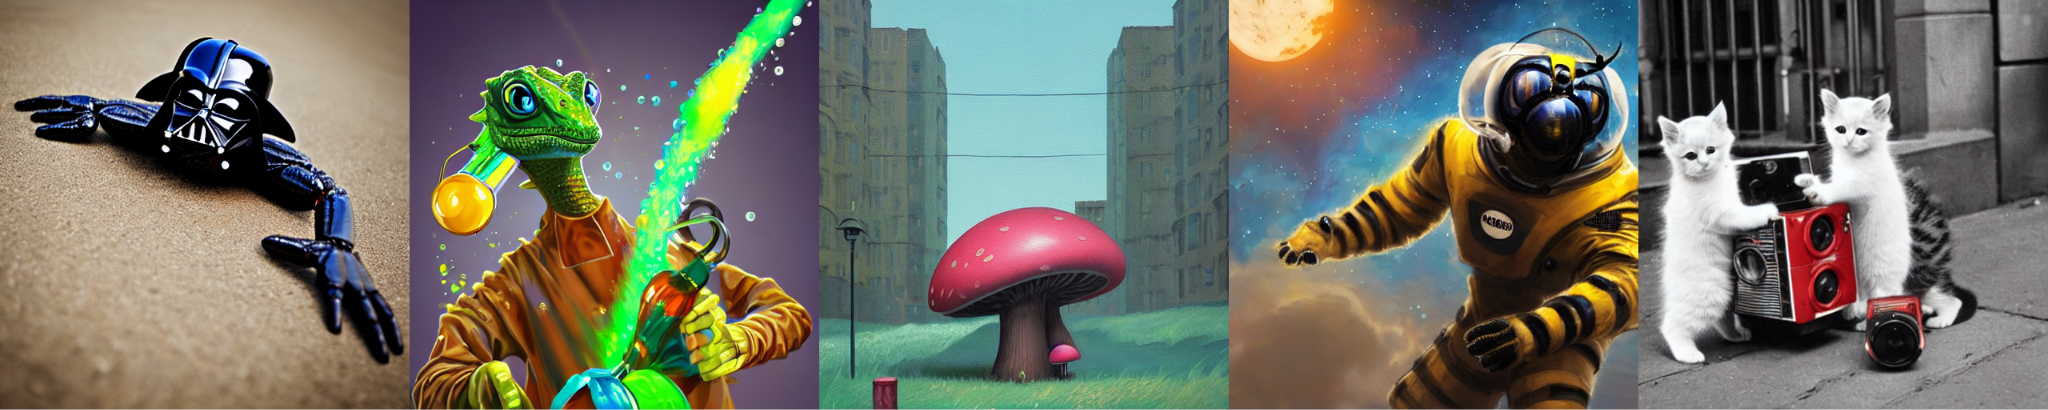
\includegraphics[width=\linewidth,height=0.42\textheight,keepaspectratio]{images/adv-img-gen/sd_sample_images_strip.png}
        \caption*{\scriptsize Text-to-image samples from Stable Diffusion. Source: CompVis, \href{https://github.com/CompVis/stable-diffusion}{stable-diffusion} repository README (\texttt{merged-0007.png}).}
    \end{figure}
    
    \framebreak

    \textbf{Advantages}
    \begin{itemize}
        \item High-quality, diverse image generation.
        \item Efficient training and inference due to latent space operations.
        \item Open weights, so the model can be inspected, fine-tuned and redistributed.
    \end{itemize}

    \framebreak

    \textbf{What do we need to make a good generative model?}
    \begin{enumerate}
        \item Method of learning to generate new images \hfill \textbf{Forward/reverse diffusion}
        \item Way to link text and images \hfill \textbf{Text-image representation model}
        \item Way to compress images \hfill \textbf{Autoencoder}
        \item Way to add in good inductive biases \hfill \textbf{U-net architecture} $+$ \textbf{`attention'}
    \end{enumerate}
    \vspace{1em}
    \textit{Making a ‘good’ generative model is about making all these parts work together well!}
\end{frame}
